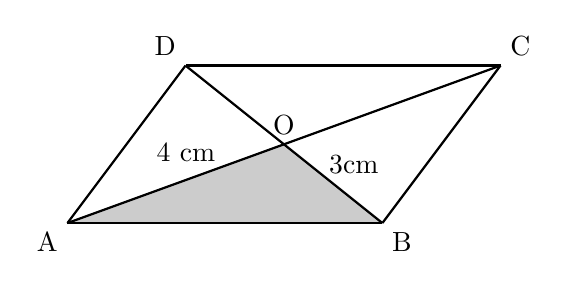
\begin{tikzpicture}

    % Define the coordinates for rhombus ABCD
    \coordinate (A) at (0, 0);       % Bottom left vertex
    \coordinate (B) at (4, 0);       % Bottom right vertex
    \coordinate (C) at (5.5, 2);     % Top right vertex
    \coordinate (D) at (1.5, 2);     % Top left vertex
    
    % Calculate the intersection point O of diagonals
    \coordinate (O) at (2.75, 1);    % Center point where diagonals meet
    
    % Draw the shaded triangle AOB with simple fill
    \fill[black!20] (A) -- (O) -- (B) -- cycle;
    
    % Draw the rhombus sides
    \draw[thick] (A) -- (B);         % Side AB
    \draw[thick] (B) -- (C);         % Side BC
    \draw[thick] (C) -- (D);         % Side CD
    \draw[thick] (D) -- (A);         % Side DA
    
    % Draw the diagonals
    \draw[thick] (A) -- (C);         % Diagonal AC
    \draw[thick] (D) -- (B);         % Diagonal DB
    
    % Label point A
    \node[below left] at (A) {A};
    
    % Label point B
    \node[below right] at (B) {B};
    
    % Label point C
    \node[above right] at (C) {C};
    
    % Label point D
    \node[above left] at (D) {D};
    
    % Label point O
    \node[above] at (O) {O};
    
    % Label the measurement 4 cm (from A to O along diagonal)
    \node[left] at (2, 0.9) {4 cm};
    
    % Label the measurement 3cm (from O to B along diagonal)
    \node[above right] at (3.2, 0.5) {3cm};
    
    \end{tikzpicture}